\section{Livres de sorts}\label{livres-de-sorts}

Les lanceurs de sorts arcaniques (magiciens et elfes) conservent les
sorts qu'ils connaissent dans un livre de sorts.

\textbf{Nombre de sorts~:} Le grimoire d'un personnage contient
exactement le nombre de sorts qu'il est capable de mémoriser (en
fonction de sa classe et de son niveau). L'arbitre peut choisir ces
sorts ou les laisser à la décision du joueur.

\subsection{Sorts de départ}\label{sorts-de-duxe9part}

Un personnage commence le jeu avec un grimoire contenant autant de sorts
qu'il peut en mémoriser. L'arbitre peut choisir ces sorts ou laisser le
joueur en décider.

\subsection{Nouveaux sorts}\label{nouveaux-sorts}

Quand un personnage gagne un niveau d'expérience, le nombre de sorts
dans son livre augmente en même temps que sa capacité de mémorisation.
Il existe deux manières de gagner de nouveaux sorts~:

\begin{itemize}
  \item \textbf{Mentors~:} Le personnage peut consulter un mentor ou une
  guilde arcanique, qui lui enseignera le ou les nouveaux sorts. Ce
  processus prend environ une semaine de temps de jeu. Les sorts appris
  sont déterminés par l'arbitre, mais il peut aussi décider de laisser
  choisir le joueur.
  \item \textbf{Recherches~:} Il est également possible d'obtenir des sorts en
  effectuant des Recherches magiques.
\end{itemize}

\subsection{Perdre son livre de sorts}\label{perdre-son-livre-de-sorts}

Un lanceur de sorts arcaniques peut réécrire les sorts d'un livre perdu
ou détruit.

\begin{itemize}
  \item \textbf{Temps et coût~:} Chaque sort demande une semaine et 1 000 po
  par niveau de sort. Par exemple, réécrire deux sorts de 1er niveau et
  un sort de 2e niveau demande 4 semaines et coûte 4 000 po.
  \item \textbf{Tâche unique~:} Cette activité demande une concentration
  intense. Le personnage ne peut pas se consacrer à quoi que ce soit
  d'autre pendant la période de réécriture des sorts.
\end{itemize}

\subsection{Livres de sorts trouvés}\label{livres-de-sorts-trouvuxe9s}

Seul le propriétaire d'un livre de sorts est capable de le lire sans
faire usage de magie (avec un sort de lecture de la magie, par exemple).

\begin{center}
  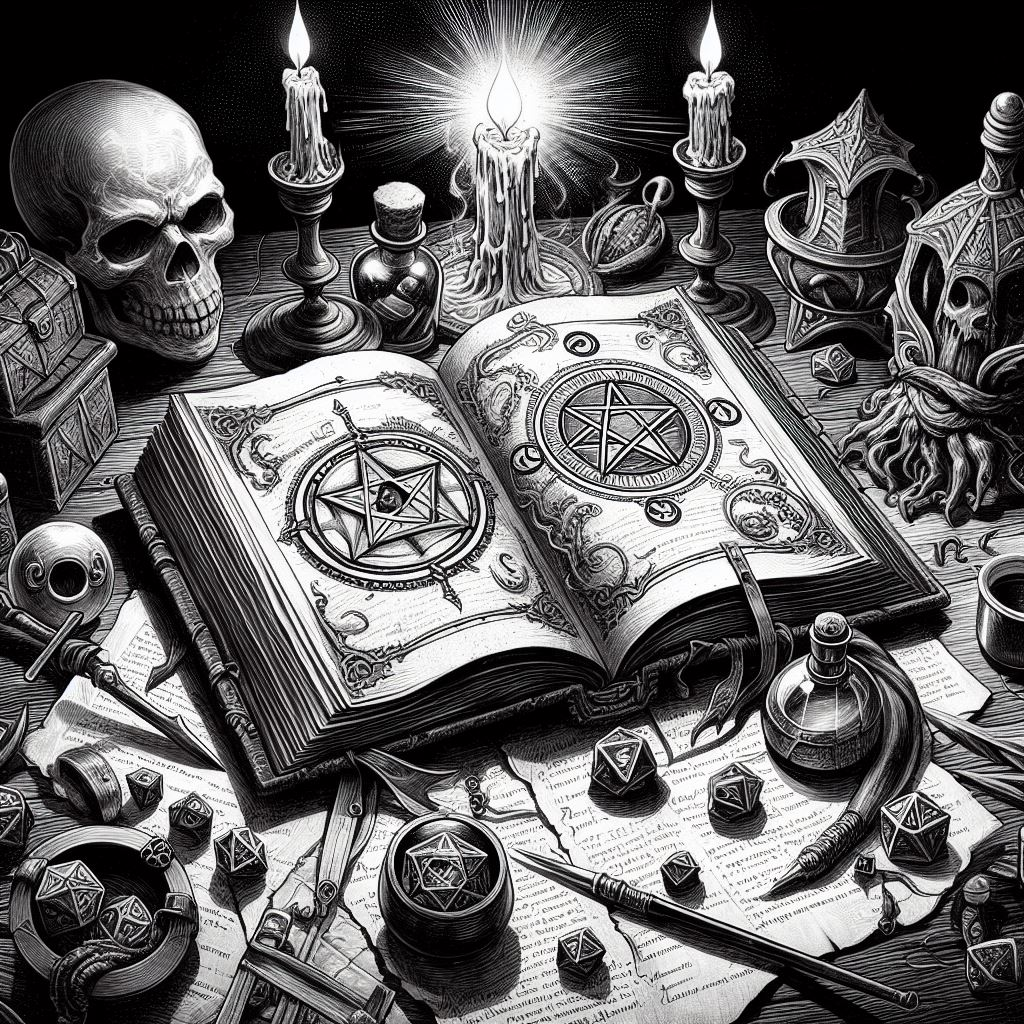
\includegraphics[width=0.75\columnwidth]{img/spellbook.jpg}
\end{center}
